Chapter 5

\chapter{Recommendation System} % Main chapter title

\label{Chapter5} % For referencing the chapter elsewhere, use \ref{Chapter1} 

\lhead{Chapter 5. \emph{Recommendation System}} % This is for the header on each page - perhaps a shortened title

%----------------------------------------------------------------------------------------

\section{Introduction}
Recommender systems became an important research area since the appearance of the first papers on collaborative filtering since the mid-1990s [45, 86, 97]. There has been much work done both in the industry and academia on developing new approaches to recommender systems over the last decade. The interest in this area still remains high because it constitutes a problem-rich research area and because of the abundance of practical applications that help users to deal with information overload and provide personalized recommendations, content and services to them. Examples of such applications include recommending books, CDs and other products at Amazon.com [61], movies by MovieLens [67], and news at VERSIFI Technologies (formerly AdaptiveInfo.com) [14]. Moreover, some of the vendors have incorporated recommendation capabilities into their commerce servers [78].

\section{Recommendation Problem}
The recommendation problem is reduced to the problem of estimating ratings for the items that have not been seen by a user. Intuitively, this estimation is usually based on the ratings given by this user to other items and on some other information that will be formally described below. Once we can estimate ratings for the yet unrated items, we can recommend to the user the item(s) with the highest estimated rating(s).
More formally, the recommendation problem can be formulated as follows. Let C be the set of all users and let S be the set of all possible items that can be recommended, such as books, movies, or restaurants. The space S of possible items can be very large, ranging in hundreds of thousands or even millions of items in some applications, such as recommending books or CDs.
Similarly, the user space can also be very large – millions in some cases. Let u be a utility function that measures usefulness of item s to user c, i.e., u :C × S → R , where R is a totally ordered set (e.g., non-negative integers or real numbers within a certain range). Then for each user c∈C , we want to choose such item s'∈S that maximizes the user’s utility. More formally
∀c∈C,  sc'=argmaxuc,ss ∈ S              (1)
In recommender systems the utility of an item is usually represented by a rating, which indicates how a particular user liked a particular item, e.g., John Doe gave the movie “Harry Potter” the rating of 7 (out of 10). However, as indicated earlier, in general utility can be an arbitrary function, including a profit function. Depending on the application, utility u can either be specified by the user, as is often done for the user-defined ratings, or is computed by the application, as can be the case for a profit-based utility function.
Each element of the user space C can be defined with a profile that includes various user characteristics, such as age, gender, income, marital status, etc. In the simplest case, the profile can contain only a single (unique) element, such as User ID. Similarly, each element of the item space S is defined with a set of characteristics. For example, in a movie  recommendation application, where S is a collection of movies, each movie can be represented not only by its ID, but also by its title, genre, director, year of release, leading actors, etc.
The central problem of recommender systems lies in that utility u is usually not defined on the whole C× S space, but only on some subset of it. This means u needs to be extrapolated to the whole space C× S . In recommender systems, utility is typically represented by ratings and is initially defined only on the items previously rated by the users. For example, in a movie recommendation application (such as the one at MovieLens.org), users initially rate some subset of movies that they have already seen. An example of a user-item rating matrix for a movie recommendation application is presented in Table 1, where ratings are specified on the scale of 1 to 5. The “∅” symbol for some of the ratings in Table 1 means that the users have not rated the corresponding movies. Therefore, the recommendation engine should be able to estimate (predict) the ratings of the non-rated movie/user combinations and issue appropriate recommendations based on these predictions.
\begin{figure}[htbp]
	\centering
		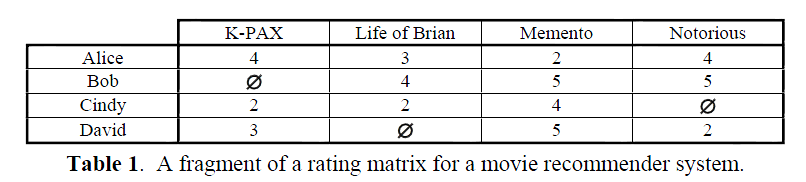
\includegraphics{./Figures/Capture.PNG}
		\rule{35em}{0.5pt}
	\caption[Angle Between Documents]{Angle Between Documents}
	\label{fig:Angle Between Documents}
\end{figure}

Extrapolations from known to unknown ratings are usually done by:
\begin{itemize}
\item [a)] Specifying heuristics that define the utility function and empirically validating its performance
\item [b)] Estimating the utility function that optimizes certain performance criterion, such as the mean square error.
\end{itemize}

Once the unknown ratings are estimated, actual recommendations of an item to a user are made by selecting the highest rating among all the estimated ratings for that user, according to formula (1). Alternatively, we can recommend N best items to a user or a set of users to an item.
The new ratings of the not-yet-rated items can be estimated in many different ways using the methods from machine learning, approximation theory and various heuristics. Recommender systems are usually classified according to their approach to rating estimation.

Recommender systems are usually classified into the following categories, based on how recommendations are made:
\begin{itemize}
\item Content-based recommendations: the user is recommended items similar to the ones the user preferred in the past
\item Collaborative recommendations: the user is recommended items that people with similar tastes and preferences liked in the past
\item Hybrid approaches: these methods combine collaborative and content-based methods
\end{itemize}

\section*{Content-based Methods}
In content-based recommendation methods, the utility u(c, s) of item s for user c is estimated based on the utilities u(c ,si)  assigned by user c to items si∈S that are "similar" to item s. For example, in a movie recommendation application, in order to recommend movies to user c, the content-based recommender system tries to understand the commonalities among the movies user c has rated highly in the past (specific actors, directors, genres, subject matter, etc.). Then, only the movies that have a high degree of similarity to whatever user’s preferences are would get recommended.
The content-based approach to recommendation has its roots in information retrieval [7,89] and information filtering [10] research. Because of the significant and early advancements made by the information retrieval and filtering communities and because of the importance of several text-based applications, many current content-based systems focus on recommending items containing textual information, such as documents, Web sites (URLs), and Usenet news messages. The improvement over the traditional information retrieval approaches comes from the use of user profiles that contain information about users’ tastes, preferences, and needs. The profiling information can be elicited from users explicitly, e.g., through questionnaires, or implicitly – learned from their transactional behavior over time.
More formally, let Content(s) be an item profile, i.e., a set of attributes characterizing item s. It is usually computed by extracting a set of features from item s (its content) and is used to determine appropriateness of the item for recommendation purposes. Since, as mentioned earlier, content-based systems are designed mostly to recommend text-based items, the content in these systems is usually described with keywords. For example, a content-based component of the Fab system [8], which recommends Web pages to users, represents Web page content with the 100 most important words. Similarly, the Syskill & Webert system [77] represents documents with the 128 most informative words. The "importance" (or "informativeness") of word ki in document dj is determined with some weighting measure wij that can be defined in several different ways.
One of the best-known measures for specifying keyword weights in Information Retrieval is the term frequency/inverse document frequency (TF-IDF) measure [89] that is defined as follows. Assume that N is the total number of documents that can be recommended to users and that keyword ki appears in ni of them. Moreover, assume that fi,j  is the number of times keyword ki appears in document dj. Then TFi,j , the term frequency (or normalized frequency) of keyword ki in document dj, is defined as
TFi,j=fi,jmaxzfz,j           (2)
Where the maximum is computed over the frequencies fz,j of all keywords kz that appear in the document dj. However, keywords that appear in many documents are not useful in distinguishing between a relevant document and a non-relevant one. Therefore, the measure of inverse document frequency (IDFi) is often used in combination with simple term frequency (TF i, j). The inverse document frequency for keyword ki is usually defined as
IDFi=logNni            (3)
Then the TF-IDF weight for keyword ki in document dj is defined as
wi,j=TFi,j×IDFi            (4)
and the content of document dj is defined as Content(dj) = (w1j, …wkj).
As stated earlier, content-based systems recommend items similar to those that a user liked in the past [56, 69, 77]. In particular, various candidate items are compared with items previously rated by the user, and the best-matching item(s) are recommended. More formally, let ContentBasedProfile(c) be the profile of user c containing tastes and preferences of this user. These profiles are obtained by analyzing the content of the items previously seen and rated by the user and are usually constructed using keyword analysis techniques from information retrieval. For example, ContentBasedProfile(c) can be defined as a vector of weights (wc1,…,wck), where each weight wci denotes the importance of keyword ki to user c and can be computed from individually rated content vectors using a variety of techniques. For example, some averaging approach, such as Rocchio algorithm [85], can be used to compute ContentBasedProfile(c) as an "average" vector from an individual content vectors [8, 56]. On the other hand, [77] use a Bayesian classifier in order to estimate the probability that a document is liked. The Winnow algorithm [62] has also been shown to work well for this purpose, especially in the situations where there are many possible features [76].
In content-based systems, the utility function u(c, s) is usually defined as:
uc, s= scoreContentBasedProfilec,Contents               (5)
Using the above-mentioned information retrieval-based paradigm of recommending Web pages, Web site URLs, or Usenet news messages, both ContentBasedProfile(c) of user c and Content(s) of document s can be represented as TF-IDF vectors Wc and WS of keyword weights. Moreover, utility function u(c, s) is usually represented in information retrieval literature by some scoring heuristic defined in terms of vectors Wc and WS , such as cosine similarity measure [7, 89]:
uc,s=cosWc , WS =Wc . WS ||Wc||2 ×||WS||2 =i=1kwi,cwi,si=1kwi,c2i=1kwi,s2         (6)
where K is the total number of keywords in the system.
For example, if user c reads many online articles on the topic of bioinformatics, then content-based recommendation techniques will be able to recommend other bioinformatics articles to user c. This is the case, because these articles will have more bioinformatics-related terms (e.g., “genome”, “sequencing”, “proteomics”) than articles on other topics,  and, therefore, ContentBasedProfile(c), as defined by vector wc , will represent such terms ki with high weights wic. Consequently, a recommender system using the cosine or a related similarity measure will assign higher utility u(c, s) to those articles s that have high-weighted bioinformatics terms in ws and lower utility to the ones where bioinformatics terms are weighted less.
Besides the traditional heuristics that are based mostly on information retrieval methods, other techniques for content-based recommendation have also been used, such as Bayesian classifiers [70, 77] and various machine learning techniques, including clustering, decision trees, and artificial neural networks [77]. These techniques differ from information retrieval-based approaches in that they calculate utility predictions based not on a heuristic formula,  such as a cosine similarity measure, but rather are based on a model learned from the underlying data using statistical learning and machine learning techniques. For example, based on a set of Web pages that were rated as “relevant” or “irrelevant” by the user, [77] use the naïve Bayesian classifier [31] to classify unrated Web pages. More specifically, the naïve Bayesian classifier is used to estimate the following probability that page pj belongs to a certain class Ci (e.g., relevant or irrelevant) given the set of keywords k1, j , …, kn,j on that page:
PCi│K1,j&…&Kn,j                 (7)
While not explicitly dealing with providing recommendations, the text retrieval community has contributed several techniques that are being used in content-based recommender systems. One example of such technique would be the research on adaptive filtering [101, 112], which focuses on becoming more accurate at identifying relevant documents incrementally, by observing the documents one-by-one in a continuous document stream. Another example would be the work on threshold setting [84, 111], which focuses on determining the extent to which documents should match a given query in order to be relevant to the user.

\section{Limitation}
\subsection{Limited content analysis}
Content-based techniques are limited by the features that are explicitly associated with the objects that these systems recommend. Therefore, in order to have a sufficient set of features, the content must either be in a form that can be parsed automatically by a computer (e.g., text), or the features should be assigned to items manually. While information retrieval techniques work well in extracting features from text documents, some other domains have an inherent problem with automatic feature extraction. For example, automatic feature extraction methods are much harder to apply to the multimedia data, e.g., graphical images, audio and video streams. Moreover, it is often not practical to assign attributes by hand due to limitations of resources [97].
Another problem with limited content analysis is that, if two different items are represented by the same set of features, they are indistinguishable. Therefore, since text-based documents are usually represented by their most important keywords, content-based systems cannot distinguish between a well-written article and a badly written one, if they happen to use the same terms [97].

\subsection{Over-specialization}
When the system can only recommend items that score highly against a user’s profile, the user is limited to being recommended items similar to those already rated. For example, a person with no experience with Greek cuisine would never receive a recommendation for even the greatest Greek restaurant in town. This problem, which has also been studied in other domains, is often addressed by introducing some randomness. For example, the use of genetic algorithms has been proposed as a possible solution in the context of information filtering [98]. In addition, the problem with over-specialization is not only that the content-based systems cannot recommend items that are different from anything the user has seen before. In certain cases, items should not be recommended if they are too similar to something the user has already seen, such as different news article describing the same event. Therefore, some content based recommender systems, such as DailyLearner [13], filter out items not only if they are too different from user’s preferences, but also if they are too similar to something the user has seen before. Furthermore, [112] provide a set of five redundancy measures to evaluate whether a document that is deemed to be relevant contains some novel information as well. In summary, the diversity of recommendations is often a desirable feature in recommender systems. Ideally, the user should be presented with a range of options and not with a homogeneous set of alternatives. For example, it is not necessarily a good idea to recommend all movies by Woody Allen to a user who liked one of them.


\subsection{New user problem}
The user has to rate a sufficient number of items before a content-based recommender system can really understand user’s preferences and present the user with reliable recommendations. Therefore, a new user, having very few ratings, would not be able to get accurate recommendations.

\section{Collaborative Methods}
Unlike content-based recommendation methods, collaborative recommender systems (or collaborative filtering systems) try to predict the utility of items for a particular user based on the items previously rated by other users. More formally, the utility u(c, s) of item s for user c is estimated based on the utilities u(cj, s) assigned to item s by those users cj∈C who are "similar" to user c. For example, in a movie recommendation application, in order to recommend movies to user c, the collaborative recommender system tries to find the "peers" of user c, i.e., other users that have similar tastes in movies (rate the same movies similarly). Then, only the movies that are most liked by the “peers” of user c would get recommended.
There have been many collaborative systems developed in the academia and the industry.It can be argued that the Grundy system [87] was the first recommender system, which proposed to use stereotypes as a mechanism for building models of users based on a limited amount of information on each individual user. Using stereotypes, the Grundy system would build individual user models and use them to recommend relevant books to each user. Later on, the Tapestry system relied on each user to identify like-minded users manually [38]. GroupLens [53, 86], Video Recommender [45], and Ringo [97] were the first systems to use collaborative filtering algorithms to automate prediction. Other examples of collaborative recommender systems include the book recommendation system from Amazon.com, the PHOAKS system that helps people find relevant information on the WWW [103], and the Jester system that recommends jokes [39].

\subsection{Collaborative recommendations algorithms}
According to [15], algorithms for collaborative recommendations can be grouped into two general classes: memory-based (or heuristic-based) and model-based. Memory-based algorithms [15, 27, 72, 86, 97] essentially are heuristics that make rating predictions based on the entire collection of previously rated items by the users. That is, the value of the unknown rating rc,s for user c and item s is usually computed as an aggregate of the ratings of some other (usually the N most similar) users for the same item s:
rc,s=aggrc'∈C rc',s            (9)
where C denotes the set of N users that are the most similar to user c and who have rated item s (N can range anywhere from 1 to the number of all users). Some examples of the aggregation function are:
arc,s= 1Nc'∈Crc',s
brc,s= kc'∈Csim(c,c')×rc',s
crc,s=rc+ kc'∈Csim(c,c')×(rc',s- rc')

where multiplier k serves as a normalizing factor and is usually selected as k= 1c'∈C|sim(c,c')| and , and where the average rating of user c, rc in (10c) is defined as
rc=1|sc|s∈Scrc,s where Sc=s∈S rc,s≠∅   (11) 
In the simplest case, the aggregation can be a simple average, as defined by expression (10a).However, the most common aggregation approach is to use the weighted sum, shown in (10b).The similarity measure between the users c and c’, sim(c, c’), is essentially a distance measure and is used as a weight, i.e., the more similar users c and c’ are, the more weight rating rc’,s will carry in the prediction of rc,s. Note that sim(x,y) is a heuristic artifact that is introduced in order to be able to differentiate between levels of user similarity (i.e., to be able to find a set of “closest peers” or “nearest neighbors” for each user) and at the same time simplify the rating estimation procedure. As shown in (10b), different recommendation applications can use their own user similarity measure, as long as the calculations are normalized using the normalizing factor k, as shown above. The two most commonly used similarity measures will be described below. One problem with using the weighted sum, as in (10b), is that it does not take into account the fact that different users may use the rating scale differently. The adjusted weighted sum, shown in (10c), has been widely used to address this limitation. In this approach, instead of using the absolute values of ratings, the weighted sum uses their deviations from the average rating of the corresponding user.


\subsection{Computing similarity between users}
Various approaches have been used to compute the similarity sim(c,c') between users in collaborative recommender systems. In most of these approaches, the similarity between two users is based on their ratings of items that both users have rated. The two most popular approaches are correlation and cosine-based. To present them, let Sxy be the set of all items co-rated by both users x and y, i.e. sxy={s∈S|rx,s≠∅ & ry,s≠∅ }. In collaborative recommender systems Sxy is used mainly as an intermediate result for calculating the "nearest neighbors" of user x and is often computed in a straightforward manner, i.e., by computing the intersection of sets Sx and Sy. However, some methods, such as the graph-theoretic approach to collaborative filtering [4], can determine the nearest neighbors of x without computing Sxy for all users y.

\subsubsection{Correlation based similarity}
In the correlation-based approach, the Pearson correlation coefficient is used to measure the similarity [86, 97]:
simx,y=s∈Sxyrx,s-rxry,s-rys∈Sxy(rx,s-rx)2s∈Sxy(ry,s-ry)2         (12)

\subsubsection{Cosine based similarity}
In the cosine-based approach [15, 91], the two users x and y are treated as two vectors in m-dimensional space, where m=|Sxy |. Then, the similarity between two vectors can be measured by computing the cosine of the angle between them:
sim(x,y)=cosx , y =x . y ||x||2 ×||y||2 =i=1krx,sry,ss∈Sxyrx,c2s∈Sxyry,s2         (13)
where x . y  denotes the dot-product between the vectors x and y . Still another approach  to measuring similarity between users uses the mean squared difference measure and is described in [97]. Note that different recommender systems may take different approaches in order to implement the user similarity calculations and rating estimations as efficiently as possible.
Many performance-improving modifications, such as default voting, inverse user frequency, case amplification [15], and weighted-majority prediction [27, 72], have been proposed as extensions to these standard correlation-based and cosine-based techniques.
\subsection{Default Voting}
an extension to the memory-based approaches described above. It was observed that whenever there are relatively few user-specified ratings, these methods would not work well in computing similarity between users x and y since the similarity measure is based on the intersection of the itemsets, i.e., sets of items rated by both users x and y .It was empirically shown that the rating prediction accuracy could improve if we assume some default rating value for the missing ratings [15].

Also, while the above techniques traditionally have been used to compute similarities between users, [91] proposed to use the same correlation-based and cosine-based techniques to compute similarities between items instead and obtain the ratings from them. This idea has been further extended in [29] for top-N item recommendations. In addition, [29, 91] present empirical evidence that item-based algorithms can provide better computational performance than traditional user-based collaborative methods, while at the same time providing comparable or better quality than the best available user-based algorithms.
In contrast to memory-based methods, model-based algorithms [11, 15, 37, 39, 47, 64, 75, 105] use the collection of ratings to learn a model, which is then used to make rating predictions. For example, [15] proposes a probabilistic approach to collaborative filtering, and it is assumed that rating values are integers between 0 and n, and the probability expression is the probability that user c will give a particular rating to item s given that user’s ratings of the previously rated items. To estimate this probability, [15] proposes two alternative probabilistic models: cluster models and Bayesian networks.

\subsection{Cluster models}
Like-minded users are clustered into classes. Given the user’s class membership, the user ratings are assumed to be independent, i.e., the model structure is that of a naïve Bayesian model. The number of classes and the parameters of the model are learned from the data.
One limitation of this approach is that each user can be clustered into a single cluster, whereas some recommendation applications may benefit from the ability to cluster users into several categories at once. For example, in a book recommendation application, a user may be interested in one topic (e.g., programming) for work purposes and a completely different topic (e.g., fishing) for leisure.

\subsection{Bayesian networks}
Represents each item in the domain as a node in a Bayesian network, where the states of each node correspond to the possible rating values for each item. Both the structure of the network and the conditional probabilities are learned from the data.

\subsection{Limitation}
\subsubsection{New user problem}
It is the same problem as with content-based systems. In order to make accurate recommendations, the system must first learn the user’s preferences from the ratings that the user makes. Several techniques have been proposed to address this problem. Most of them use hybrid recommendation approach, which combines content-based and collaborative techniques. The next section describes hybrid recommender systems in more detail. An alternative approach is presented in [83, 109], where various techniques are explored for determining the best (i.e., most informative to a recommender system) items for a new user to rate. These techniques use strategies that are based on item popularity, item entropy, user personalization, and combinations of the above [83, 109].

\subsubsection{New item problem}
New items are added regularly to recommender systems. Collaborative systems rely solely on users’ preferences to make recommendations. Therefore, until the new item is rated by a substantial number of users, the recommender system would not be able to recommend it.

\subsubsection{Sparsity}
In any recommender system, the number of ratings already obtained is usually very small compared to the number of ratings that need to be predicted. Effective prediction of ratings from a small number of examples is important. Also, the success of the collaborative recommender system depends on the availability of a critical mass of users. For example, in the movie recommendation system there may be many movies that have been rated only by few people and these movies would be recommended very rarely, even if those few users gave high ratings to them. Also, for the user whose tastes are unusual compared to the rest of the population there will not be any other users who are particularly similar, leading to poor recommendations [8]. One way to overcome the problem of rating sparsity is to use user profile information when calculating user similarity. That is, two users could be considered similar not only if they rated the same movies similarly, but also if they belong to the same demographic segment. For example, [76] uses gender, age, area code, education, and employment information of users in the restaurant recommendation application. This extension of traditional collaborative filtering techniques is sometimes called “demographic filtering” [76]. Another approach that also explores similarities among users has been proposed in [49], where the sparsity problem is addressed by applying associative retrieval framework and related spreading activation algorithms to explore transitive associations among consumers through their past transactions and feedback. A different approach for dealing with sparse rating matrices was used in [11, 90], where a dimensionality reduction technique, Singular Value Decomposition (SVD), was used to reduce dimensionality of sparse ratings matrices. SVD is a well-known method for matrix factorization that provides the best lower rank approximations of the original matrix [90].

\section{Hybrid Methods}
Several recommendation systems use a hybrid approach by combining collaborative and content-based methods, which helps to avoid certain limitations of content-based and collaborative systems. Different ways to combine collaborative and content-based methods into a hybrid recommender system can be classified as follows:
\begin{itemize}
\item [1] Implementing collaborative and content-based methods separately and combining their predictions
\item [2] incorporating some content-based characteristics into a collaborative approach
\item [3] incorporating some collaborative characteristics into a content-based approach
\item [4] constructing a general unifying model that incorporates both content-based and collaborative characteristics.
\end{itemize}

\subsection{Combining separate recommenders}
One way to build hybrid recommender systems is to implement separate collaborative and content-based systems. Then we can have two different scenarios.
First, we can combine the outputs (ratings) obtained from individual recommender systems into one final recommendation using either a linear combination of ratings [21] or a voting scheme [76]. 
Alternatively, we can use one of the individual recommenders, at any given moment choosing to use the one that is "better" than others based on some recommendation "quality" metric 
For example, the DailyLearner system [13] selects the recommender system that can give the recommendation with the higher level of confidence, while [104] chooses the one whose recommendation is more consistent with past ratings of the user.

\subsection{Adding content-based characteristics to collaborative models}
Several hybrid recommender systems, including Fab [8] and the “collaboration via content” approach, described in [76], are based on traditional collaborative techniques but also maintain the content-based profiles for each user. These content-based profiles, and not the commonly rated items, are then used to calculate the similarity between two users. As mentioned in [76], this allows to overcome some sparsity-related problems of a purely collaborative approach, since typically not many pairs of users will have a significant number of commonly rated items. Another benefit of this approach is that users can be recommended an item not only when this item is rated highly by users with similar profiles, but also directly, i.e., when this item scores highly against the user’s profile [8]. [40] employs a somewhat similar approach in using the variety of different filterbots – specialized content-analysis agents that act as additional participants in a collaborative filtering community. As a result, the users whose ratings agree with some of the filterbots’ ratings would be able to receive better recommendations [40]. Similarly, [65] uses a collaborative approach where the traditional user’s ratings vector is augmented with additional ratings, which are calculated using a pure content-based predictor.

\subsection{Adding collaborative characteristics to content-based models}
The most popular approach in this category is to use some dimensionality reduction technique on a group of content-based profiles. For example, [100] use latent semantic indexing (LSI) to create a collaborative view of a collection of user profiles, where user profiles are represented by term vectors  resulting in a performance improvement.

\subsection{Developing a single unifying recommendation model}
Many researchers have followed this approach in recent years. For instance, [9] propose to use content-based and collaborative characteristics (e.g., the age or gender of users or the genre of movies) in a single rule-based classifier. [80] And [94] propose a unified probabilistic method for combining collaborative and content-based recommendations, which is based on the probabilistic latent semantic analysis [46]. Yet another approach is proposed by [25] and [5], where Bayesian mixed-effects regression models are used that employ Markov chain Monte Carlo methods for parameter estimation and prediction.

\section{Demographic-based Methods}
Demographic information can be used to identify the types of users that like a certain object. For example, Table 3 shows information on the age, gender, education, etc. of people that rated a restaurant together with their rating of the restaurant. One might expect to learn the type of person that likes a certain restaurant. Similarly, Lifestyle Finder (Kruwlich 1997) attempts to identify one of 62 pre-existing clusters to which a user belongs and to tailor recommendations to user based upon information about others in the cluster. Obtaining demographic information can be difficult. Lifestyle Finder enters into dialog with the user to help categorize the user.
In this work, we consider an alternative approach to obtaining demographic information in which we minimize the effort required to obtain information about users by leveraging the work the user has already expended in creating a home page on the World Wide Web . Therefore, instead of using approaches to learning from a structured database, we use text classification to classify users. The positive examples are the HTML home pages of users that like a particular restaurant and the negative examples are the HTML home pages of users that do not like that restaurant. The Winnow algorithm can be used to learn the characteristics of home pages associated with users that like a particular restaurant. While it might be preferable to obtain (or extract) structured information about users, we argue that there is a trade-off between the quality of the demographic information obtained and the amount of effort required to obtain it.

\section{Collaboration via content}
Collaborative methods look for similarities between users to make predictions. Typically, the pattern of ratings of individual users is used to determine similarity. Such a correlation is most meaningful when there are many objects rated in common between users.
The content-based profile of each user is exploited to detect similarities among users. Recall that the user’s content-based profile contains weights for the terms that indicate that a user will like an object. Before calculating the similarity between profiles, terms that are irrelevant are deleted from each profile. This avoids considering two users to be very similar if they share a large number of terms that are irrelevant and have low weights. When computing Pearson’s r between two profiles, any word in one profile but not another is treated as having a weight of 0 in the other profile. As in collaborative filtering, the prediction made is determined by a weighted average of all user’s predictions for that item using the correlation between profiles as the weight.

\section{Building user Profile}
For the content-based approach which we are taking, there are four essential requirements:

FEE TABLE HENA

The assumption underlying content-based systems is that the content (rather than appearance, interactivity, speed of loading, etc.) of a page is what determines the user's interest. Now we make the further assumption that we can represent the content of a page purely by considering the words contained in the text. We ignore all mark-up tags, images and other multimedia information.
The vector-space model of information retrieval (Salton & McGill 1983) provides us with an appropriate representation for documents based on their constituent words. This model has been used and studied extensively, forms the basis for commercial web search systems and has been shown to be competitive with alternative IR methods (Harman 1995).
In this model documents and queries are represented as vectors. Assume some dictionary vector d, where each element di is a word. Each document then has a vector w, where element wi is the weight of word di for that document. If the document does not contain di then wi = 0.
In our formulation we reduce words to their stems, ignore words from a stop list words, and calculate a TFIDF weight.
In an attempt to avoid over-fitting, and reduce memory and communications load, we use just the 100 highest-weighted words from any document. Recent experiments described in (Pazzani, Muramatsu, & Billsus 1996) have shown that using too many words leads to a decrease in performance when classifying web pages using supervised learning methods. So, the top N informative words are chosen using TFIDF weighting to determine them.
Once the top N words have been picked we normalize w to be of unit length, to allow comparisons between documents of different lengths.
This vector representation is used both for pages, as explained, and for the model of the user's interests, the user profile m (which corresponds to the query in a retrospective IR system). In order to measure how well a page w matches a profile m, we use a variant of the standard IR cosine measure:
rw,m= w.m
Updating m also corresponds to a normal operation in retrospective IR: relevance feedback (Rocchio 1971).We use a simple update rule:
u(w,m,s) =m+sw
where s is the user's score for page w (we translate the scale shown in following Figure to the integers 3, 2, 1, 0, -1,-2, -3).
\begin{figure}[htbp]
	\centering
		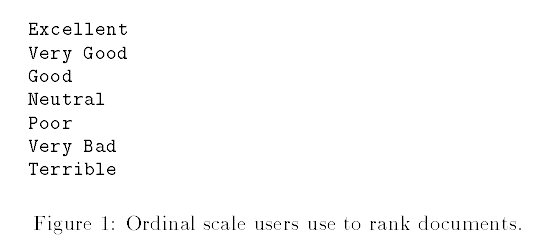
\includegraphics{./Figures/Capture2.PNG}
		\rule{35em}{0.5pt}
	\caption[Angle Between Documents]{Angle Between Documents}
	\label{fig:Angle Between Documents}
\end{figure}
We assume that a user's interests change over time, and furthermore that this happens in real time, regardless of the number of recommendations requested per day. This process is modeled using a simple decay function-each night all the weights in the profiles are multiplied by 0.97.
 
\section{User's Feedback}

\section{Collaboration via content}
\subsection{Explicit feedback}
Explicit feedback is not a good choice for two reasons. Users will have to rate items frequently and will be very reluctant in doing so as their ratings expire quickly.

\subsection{Implicit feedback}
Acquiring feedback by observing the users’ actions is favorable. A user that selects and reads a document for a certain amount of time provides a strong indication that the document contains information a user is interested in. After such action the documents is therefore classified as a positive example. Finding negative examples is much more problematic. Users ignoring links to documents could be seen as a clue. This action does not provide strong evidence however as users might not have noticed the link or visit the document later. Another possible clue is a document that is being read for a very short time but this could be caused by the fact that the document is similar to what the user has already seen although the topic of the document is still interesting to the user. Classifying documents as negative based on weak assumptions leads to much noise in the training data and may result in inaccurate predictions. Negative examples will therefore not be used. In short, the user model has to be dynamic and learned from positive examples only.
\section{Using LSA in Recommendation}
Latent semantic analysis provides a vector of a predefined length (the number of documents used in building the term versus document matrix) for representing documents.
So, we proposed using LSA vector representation to represent both documents and users profile.
\subsection{Advantage of using LSA}
\begin{itemize}
\item  The length of both user profile vector and document is the same
\item  Calculating correlation between users is done in constant time
\item  Updating user profile is done in constant time just by adding the vector of the document multiplied by user feedback to the user vector
\end{itemize}




